\subsection{Random Sample Consensus and Robust Estimation}

Given a set of 2D image features and their associated 3D map points in a world frame, it is possible to determine the unique transformation which places the camera in the world frame relative to the map points \cite{longuet-higginsComputerAlgorithmReconstructing1981}. This algorithm is known as Perspective-n-Point (PnP), and is the mechanism for localizing 2D images within the 3D map in KV-SLAM. Additionally, through methods like the eight point algorithm \cite{hartleyDefenseEightpointAlgorithm1997}, the relative camera transformation between two images, and the depths of the jointly observed points can be determined. This 2D-2D correspondence is the basis for map initialization. But as shown above, the process of extracting and matching image features is noisy, and will contain outlier data, meaning that incorrect correspondences between point can lead to an incorrect solution or no solution being found. The solution to this issue is the Random Sample Consensus algorithm.

The RANSAC algorithm is very easy to understand visually. Let's imagine a sensor measures linear data, but introduces some normally distributed noise about the true measurement. Additionally, the sensor has a bug which causes about 20 percent of the readings to be outliers. The output produced by such a sensor may look like the left most plot of Figure \ref{fig:ransac}. As can be seen, the best fit for all the data is far from correct due to the outliers. By iteratively selecting a random sample of the input data, fitting the model to this sample, and counting the number of inliers, RANSAC can find a solution which explains the highest proportion of the observations.

\begin{figure}[!ht]
    \centering
    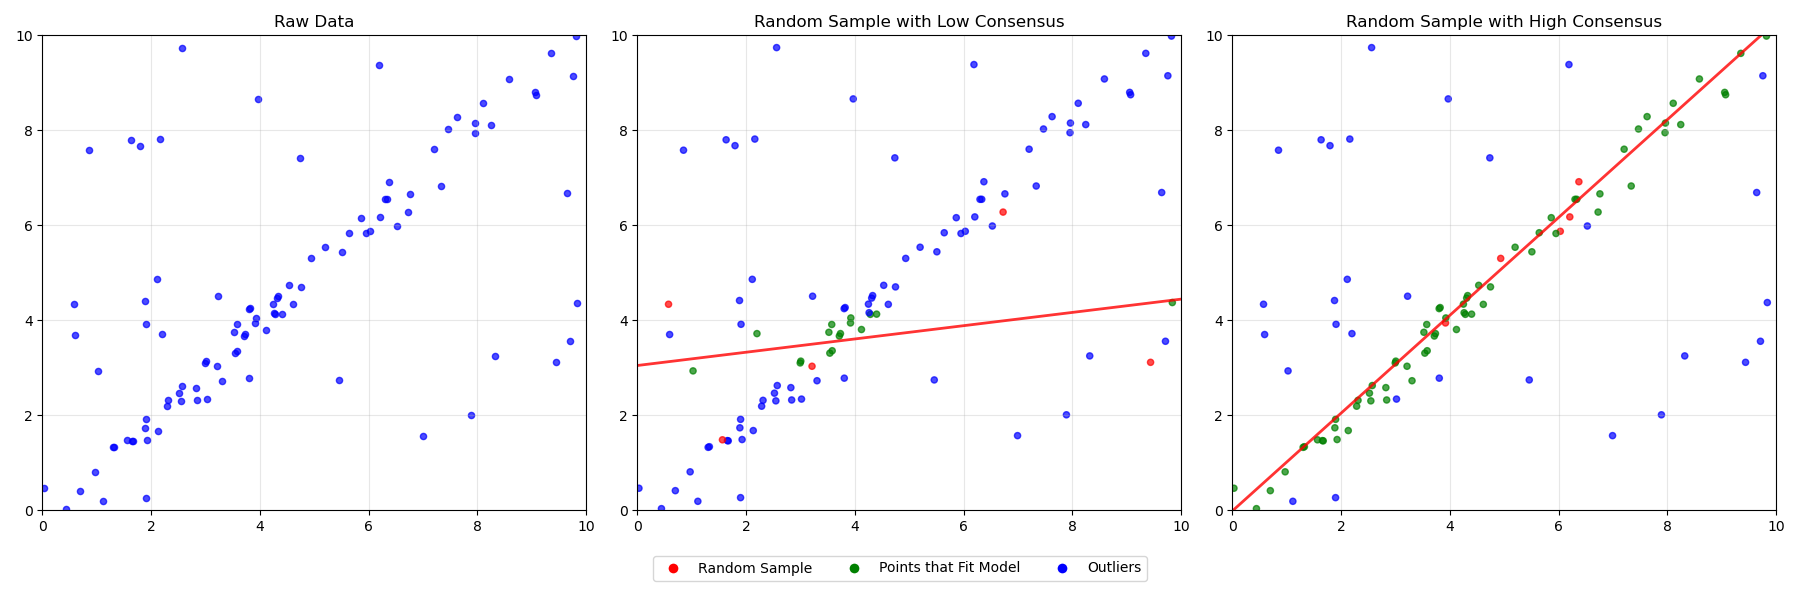
\includegraphics[width=0.9\textwidth]{resources/ransac.png}
    \caption[2D RANSAC Example]{A demonstration of how RANSAC determines model parameters through iterative random sampling and model application.}
    \label{fig:ransac}
\end{figure}